%------------------------------------------------------------------------------%
%                                   hedgehog                                   %
%------------------------------------------------------------------------------%

\section{Hedgehog}
\label{sec:hh}

\gls{hh} is a template library that uses data-flow graphs to create
parallel algorithms \cite{bardakoff2021analysis}. The library is the direct
descendent of \gls{hmbe} that also uses data-flow graphs
\cite{blattner2017model}.

In this section, we will present some of the features of the library and how
we can use it to express an algorithm under the form of a graph.

\subsection{The data-flow graphs}

As we have explained in the introduction of this section, we need to express our
algorithms under the form of data-flow graphs. A data-flow graph is a graph
where edges represent data streams and vertices represent tasks
\cite{kavi1986formal} and \cite{bardakoff2021analysis}. We can see an example of
data-flow graph on the figure \ref{fig:data-flow-graph-example}.

% TODO figure
% [Data-flow graph example] {{{
\begin{figure}[h!]
  \begin{center}
    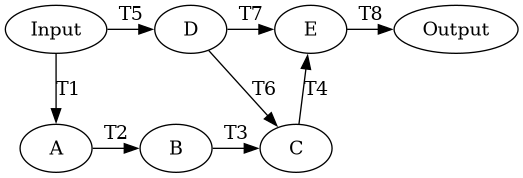
\includegraphics[scale=0.5]{./img/data-flow-graph-example.png}
    \caption{Data-flow graph example}
    \label{fig:data-flow-graph-example}
  \end{center}
\end{figure}
%}}}

In each task, the inputted data will be transformed into new data that will be
the input of other tasks. For instance, on the figure
\ref{fig:data-flow-graph-example}, we have two inputs of types \texttt{T1} and
\texttt{T5}. The data of type T1 is inputed into the task \texttt{A} that will
produce a new data of type \texttt{T2} that will be transmitted to the task
\texttt{B}. At the end of the graph, the task \texttt{E} generate a data of type
\texttt{T8} that will be the output of the graph.

In \gls{hh}, the data are transmitted between nodes using shared pointers in
order to be as efficient as possible even with big data types. % todo: reformulate

\subsection{The nodes}

To design an algorithm using Hedgehog, we have to create a graph in which the
datas will flow. A graph is composed of nodes of different kinds that we will
describe in this section.

\subsubsection{Tasks}

The first type of nodes are the tasks. These nodes are made to be duplicated and
ran in different threads. As all other nodes, a task can have multiple input and
output types.

On the listing \ref{lst:hhtask}, we can see how to create a task using \gls{hh}.
To do so, we use a class that inherits from \texttt{hh::AbstractTask} and we
override the \texttt{execute} and \texttt{copy} functions. The
\texttt{execute} functions are called when the task receives a data of a certain
type and the \texttt{copy} function is used to duplicate the task in order for
it to run on multiple threads.

The tasks have at least three template parameters. The first one is the number
of input types (in this example, we have two input types) and it is followed by
the list of the input types (T3 and T6) and the list of the output types (T4).

%- begin listing ------------------------------------------------------------{{{
\begin{listing}[ht!]
\begin{minted}[frame=lines,framesep=2mm,baselinestretch=1.2,fontsize=\normalsize,linenos]{C++}
  class C: public hh::AbstractTask<2, T6, T3, T4> {
  public:
    SubLineTask(size_t nbThreads):
        hh::AbstractTask<2, T6, T3, T4>("C", nbThreads) {}

    void execute(std::shared_ptr<T3> data) override {
      // compute with T3 data
      return std::make_shared<T4>(/* ... */)
    }

    void execute(std::shared_ptr<T6> data) override {
      // compute with T6 data
      return std::make_shared<T4>(/* ... */)
    }

    std::shared_ptr<hh::AbstractTask<2, T6, T3, T4>>
    copy() override {
        return std::make_shared<C>(this->numberThreads());
    }
};
\end{minted}
\captionof{listing}{Hedgehog: Task}
\label{lst:hhtask}
\end{listing}
%- end listing --------------------------------------------------------------}}}

\subsubsection{States}

The states are special nodes that are only made for synchronisation and cannot
be duplicated. They are thread safe and can be used to control the data-flow in
the graph. We have to be careful when creating a state as it locks the program
using a mutex. This means that only simple operations have to be made in the
states in order not to slow the program execution.

The creation of a state is very similar to the creation of a task. A state
inherits from \texttt{hh::AbstractState} and override the \texttt{execute}
function. However, the state does not have a \texttt{copy} function since it
should not be parallelized.

A state cannot be used directly in a graph and must be controlled by a state
mamanger. We will describe this component in the section \ref{sec:statemanager}.

\subsubsection{State managers}
\label{sec:statemanager}

The state manager is a node that will own a state. It is in charge of locking
the state when it receives a new data. We can have multiple state managers
owning the same state in a graph, in the case we want to use the same state at
multiple state of the computation. \gls{hh} has a default implementation for the
state manager, but we can create our own one to handle cycles.

Indeed, one of the most interesting features of \gls{hh} is the fact that it
allows the creation of cycles in the graphs. This is particularly useful when we
want to repeat an operation multiple times (a loop in the computation). However,
it is not possible to automatically detect when we can break the cycle at
runtime. Thankfully, the user of the library can implement its own state
mamanger and override the \texttt{canTerminate} function. This function will be
used the stop the state when it is possible.

In the listing \ref{lst:statemanager} we can see an example of a state mamanger
that will own a state of type \texttt{MyState}. Here, the \texttt{canTerminate}
function is overriden to and returns if the state is finished or not. In this
function, we lock the state, and we use the \texttt{idDone} method that has been
defined in the state and that returns true when the state is done. The template
parameters of the \texttt{StateManager} should be equal to the one of the
state.

%- begin listing ------------------------------------------------------------{{{
\begin{listing}[ht!]
\begin{minted}[frame=lines,framesep=2mm,baselinestretch=1.2,fontsize=\normalsize,linenos]{C++}
  class MySM: public hh::StateManager<1, T1, T2, T3, T4> {
  public:
    MySM(std::shared_ptr<MyState> const& state):
        hh::StateManager<1, T1, T2, T3, T4>(state, "My SM") { }

    [[nodiscard]] bool canTerminate() const override {
        this->state()->lock();
        auto ret = std::dynamic_pointer_cast<MyState>(this->state())->isDone();
        this->state()->unlock();
        return ret;
    }
};
\end{minted}
\captionof{listing}{Hedgehog: state manager}
\label{lst:statemanager}
\end{listing}
%- end listing --------------------------------------------------------------}}}

\subsubsection{Graphs}

The graph itself is a node as well which means that we can use a graph in
another one. In a graph, we can create edges between different nodes in order
form them to be able to communicate.

The listing \ref{lst:graph} shows an example of a graph creation. Here we can
see that we create some nodes (task and states) and we construct the graph by
creating edges between nodes. For instance, at the line 12, we create an edge
between \texttt{myTask1} and \texttt{myTask2}, which means that the task one
(the sender) will output data to the task two (the receiver). To be able to
create an edge between two nodes, they must share at least one type (if task one
outputs a data of type \texttt{T1}, the task two should acept this type as
input). As all the other nodes, the graph as inputs and outputs, and we can use
the corresponding methods to specify which node will be used to receive or send
the data.

%- begin listing ------------------------------------------------------------{{{
\begin{listing}[ht!]
\begin{minted}[frame=lines,framesep=2mm,baselinestretch=1.2,fontsize=\normalsize,linenos]{C++}
class MyGraph: public hh::Graph<1, T1, T2> {
  public:
    GaussGraph(size_t matrixHeight, size_t nbThreads):
        hh::Graph<1, T1, T2>("My Graph") {
      auto myTask1 = std::make_shared<MyTask1>(/* nbThreads, ... */);
      auto myTask2 = std::make_shared<MyTask2>(/* nbThreads, ... */);
      auto myState = std::make_shared<MySate>(/* ... */);
      auto myStateManager = std::make_shared<MySM>(myState);

      this->inputs(myTask1);
      this->edges(mayTask1, myTaks2);
      this->edges(mayTask1, myStateManager);
      this->edges(mayTask2, myStateManager);
      this->edges(myStateManager, mayTask2);
      this->outputs(myStateManager);
    }
};
\end{minted}
\captionof{listing}{Hedgehog: graph}
\label{lst:graph}
\end{listing}
%- end listing --------------------------------------------------------------}}}

The graph class can be used to instanciate a graph to which we can push some
data as shown on the listing \ref{lst:graphusage}. Once all the objects have been
pushed to the graph, we use the function \texttt{finishPushingData} to start the
computation, and we wait for the result.

%- begin listing ------------------------------------------------------------{{{
\begin{listing}[ht!]
\begin{minted}[frame=lines,framesep=2mm,baselinestretch=1.2,fontsize=\normalsize,linenos]{C++}
MyGraph myGraph;

myGraph.executeGraph();
myGraph.pushData(/* ... */);
myGraph.finishPushingData();
myGraph.waitForTermination();
\end{minted}
\caption{Hedgehog: using a graph}
\label{lst:graphusage}
\end{listing}
%- end listing --------------------------------------------------------------}}}

\subsection{Profiling}

% example of dot file

\subsection{Example}
